\section{EXPERIMENTS AND RESULTS}
\subsection{Result from Prediction models}
In this project, various algorithms were implemented to predict the stock market. Technical analysis was done for short term prediction of individual companies, using ANN classifier, ANN regression and KNN algorithms. Likewise, News-sentimental analysis was done for short term prediction of NEPSE index using Naive Bayes algorithm, whereas, under fundamental analysis, the intrinsic valuation of a company was calculated to determine whether the price of a stock is undervalued or overvalued. The algorithms used and their respective accuracies are summarized below:

~

\begin{table}[h!]
	\centering
	\begin{tabular}{|l|l|}
	\hline
	\textbf{Prediction Model} & \textbf{Accuracy}\\
	\hline
	ANN classifier & 72\%\\
	\hline
	ANN Regression & 92\%\\
	\hline
	KNN classifier & 65\%\\
	\hline	
	Naive Bayes Classifier & 68\%\\
	\hline
	\end{tabular}
	\caption{Result from prediction models}
	\label{tab:Result from prediction models}
\end{table}

\subsection{Result from Technical Analysis}
\subsubsection{Regression using ANN}
In ANN regression, six factors were considered as input factors. They are: Open price, Close price, High price, Low price, Number of transactions, Traded volume. Comparison was done based on the number of hidden neurons. Comparison charts with actual and predicted values for NABIL bank, for 150 working days, using 20, 30 and 40 hidden neurons are shown below:

~

\begin{figure}[H]\centering
  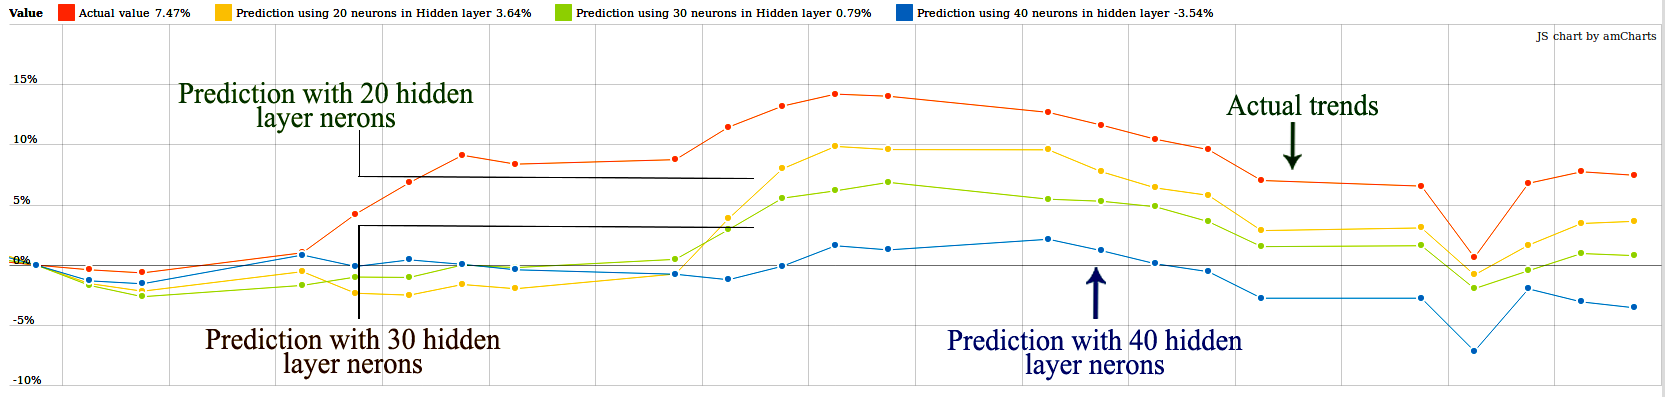
\includegraphics[width=\textwidth]{fig/prediction1}
  \caption{Result comparision for varying number of neurons in hidden layer}
  \label{fig:prediction1}
\end{figure}

The prediction model with 30 hidden neurons shows better results. 

~

\begin{figure}[H]\centering
  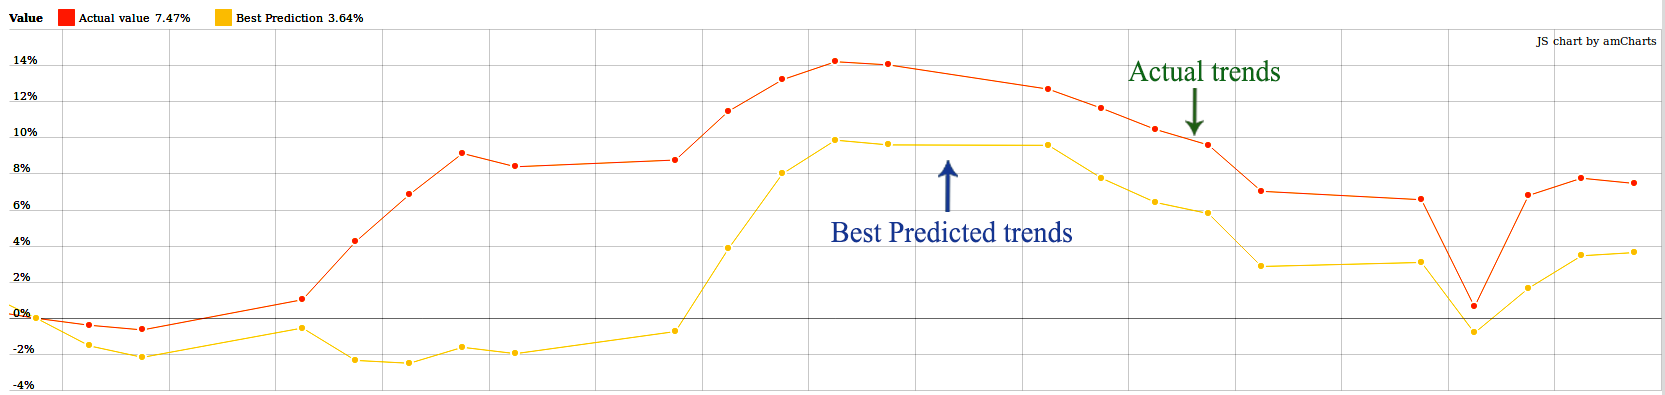
\includegraphics[width=\textwidth]{fig/pred}
  \caption{Result analysis showing 30 hidden layer neurons}
  \label{fig:pred}
\end{figure}

\subsubsection{Classification using ANN}
In this model, the trend for the next day's stock price for a company is predicted. The chart below shows the actual trends and predicted trends for NABIL bank for 100 working days.
The rise in waveform depicts the rise in stock price whereas the fall in waveform depicts the fall in stock price.

~

\begin{figure}[H]\centering
  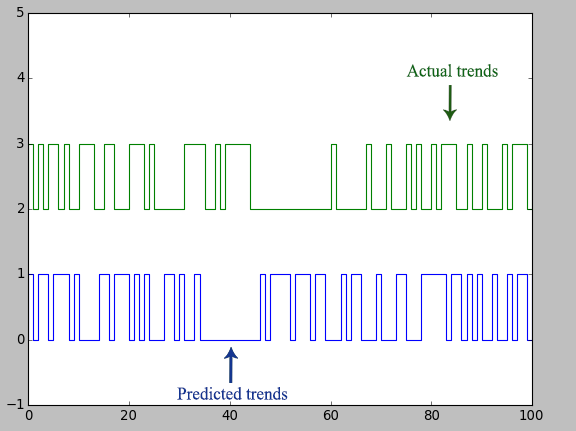
\includegraphics[width=\textwidth]{fig/ann}
  \caption{Result analysis of classification using ANN}
  \label{fig:ann}
\end{figure}

\subsubsection{Classification using KNN}
In this model, the trend for the next day's stock price for company is predicted. The chart below shows the actual trends and the predicted trends for NABIL bank for 100 working days. The rise in waveform depicts the rise in stock price whereas the fall in waveform depicts the fall in stock price.

~

\begin{figure}[H]\centering
  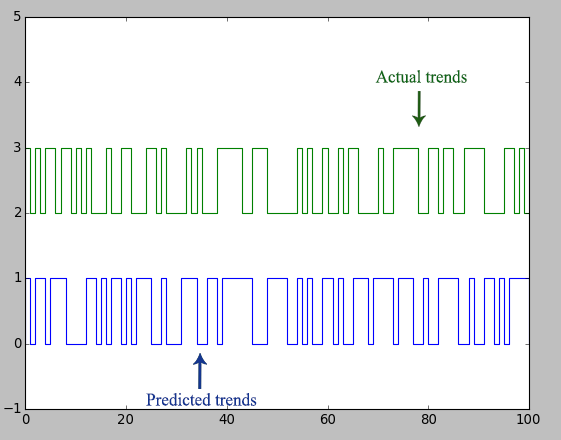
\includegraphics[width=\textwidth]{fig/knn}
  \caption{Result analysis of classification using KNN}
  \label{fig:knn}
\end{figure}

%\newpage
\subsection{Result from News Sentiment Analysis}
\subsubsection{Classification using News-sentiment}
In this model, the trend for NEPSE index is predicted. The chart below shows the actual NEPSE trend and the predicted NEPSE trend taken over a period of 100 working days. The rise in waveform depicts the rise in index whereas the fall in waveform depicts the fall in index.

~

\begin{figure}[H]\centering
  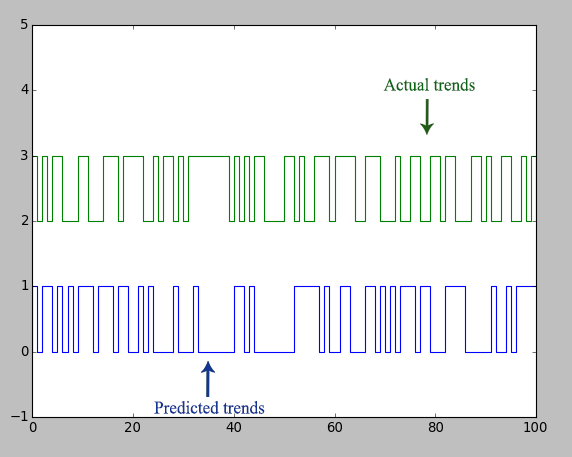
\includegraphics[width=\textwidth]{fig/news}
  \caption{Result analysis of classification using news-sentiment}
  \label{fig:news}
\end{figure}

\subsubsection{Result from Confusion Matrix}
The table \ref{tab:confusion} shows confusion matrix for Naive Bayes algorithm implemented for news analysis. The matrix was created using the news collected over 60 days.

~

\begin{table}[h!]
	\centering
	\begin{tabular}{|l|l|l|}
	\hline
	& \textbf{Predicted High} & \textbf{Predicted Low} \\
	\hline
\textbf{Actual High} & True Positive = 27 & False Negative = 9\\
	\hline
\textbf{Actual Low}	& False Positive = 10 & True Negative = 14\\
	\hline
	\end{tabular}
	\caption{Confusion Matrix for Naive Bayes Classifier}
	\label{tab:confusion}
\end{table}

~

\newpage
In table \ref{tab:Result analysis of News Sentiment}, results obtained from the confusion matrix are analyzed using various terminologies. 
 
  \begin{table}[h!]
  	\centering
  	\begin{tabular}{|l|l|}
  	\hline
	\textbf{Terminology} & \textbf{Values}\\
	\hline
	Sensitivity(True positive rate) & 0.7500\\
	\hline
	Specificity(True negative rate) & 0.5833\\
	\hline
	Precision(Positive predictive value) & 0.7297\\
	\hline
	Recall(Negative predictive value) & 0.6086\\
	\hline
	Matthews correlation coefficient & 0.3358\\
	\hline
	F1 score & 0.7397\\
	\hline
	Bookmaker informedness & 0.3333\\
	\hline
	Markedness & 0.3383\\
	\hline	
	Accuracy & 68.3300\%\\
	\hline
	\end{tabular}
    \caption{Result analysis of News Sentiment}
	\label{tab:Result analysis of News Sentiment}
  
  \end{table}






